% Options for packages loaded elsewhere
\PassOptionsToPackage{unicode}{hyperref}
\PassOptionsToPackage{hyphens}{url}
\PassOptionsToPackage{dvipsnames,svgnames,x11names}{xcolor}
%
\documentclass[
  letterpaper,
  DIV=11,
  numbers=noendperiod,
  oneside]{scrartcl}

\usepackage{amsmath,amssymb}
\usepackage{iftex}
\ifPDFTeX
  \usepackage[T1]{fontenc}
  \usepackage[utf8]{inputenc}
  \usepackage{textcomp} % provide euro and other symbols
\else % if luatex or xetex
  \usepackage{unicode-math}
  \defaultfontfeatures{Scale=MatchLowercase}
  \defaultfontfeatures[\rmfamily]{Ligatures=TeX,Scale=1}
\fi
\usepackage{lmodern}
\ifPDFTeX\else  
    % xetex/luatex font selection
\fi
% Use upquote if available, for straight quotes in verbatim environments
\IfFileExists{upquote.sty}{\usepackage{upquote}}{}
\IfFileExists{microtype.sty}{% use microtype if available
  \usepackage[]{microtype}
  \UseMicrotypeSet[protrusion]{basicmath} % disable protrusion for tt fonts
}{}
\makeatletter
\@ifundefined{KOMAClassName}{% if non-KOMA class
  \IfFileExists{parskip.sty}{%
    \usepackage{parskip}
  }{% else
    \setlength{\parindent}{0pt}
    \setlength{\parskip}{6pt plus 2pt minus 1pt}}
}{% if KOMA class
  \KOMAoptions{parskip=half}}
\makeatother
\usepackage{xcolor}
\usepackage[left=1in,marginparwidth=2.0666666666667in,textwidth=4.1333333333333in,marginparsep=0.3in]{geometry}
\setlength{\emergencystretch}{3em} % prevent overfull lines
\setcounter{secnumdepth}{-\maxdimen} % remove section numbering
% Make \paragraph and \subparagraph free-standing
\makeatletter
\ifx\paragraph\undefined\else
  \let\oldparagraph\paragraph
  \renewcommand{\paragraph}{
    \@ifstar
      \xxxParagraphStar
      \xxxParagraphNoStar
  }
  \newcommand{\xxxParagraphStar}[1]{\oldparagraph*{#1}\mbox{}}
  \newcommand{\xxxParagraphNoStar}[1]{\oldparagraph{#1}\mbox{}}
\fi
\ifx\subparagraph\undefined\else
  \let\oldsubparagraph\subparagraph
  \renewcommand{\subparagraph}{
    \@ifstar
      \xxxSubParagraphStar
      \xxxSubParagraphNoStar
  }
  \newcommand{\xxxSubParagraphStar}[1]{\oldsubparagraph*{#1}\mbox{}}
  \newcommand{\xxxSubParagraphNoStar}[1]{\oldsubparagraph{#1}\mbox{}}
\fi
\makeatother


\providecommand{\tightlist}{%
  \setlength{\itemsep}{0pt}\setlength{\parskip}{0pt}}\usepackage{longtable,booktabs,array}
\usepackage{calc} % for calculating minipage widths
% Correct order of tables after \paragraph or \subparagraph
\usepackage{etoolbox}
\makeatletter
\patchcmd\longtable{\par}{\if@noskipsec\mbox{}\fi\par}{}{}
\makeatother
% Allow footnotes in longtable head/foot
\IfFileExists{footnotehyper.sty}{\usepackage{footnotehyper}}{\usepackage{footnote}}
\makesavenoteenv{longtable}
\usepackage{graphicx}
\makeatletter
\newsavebox\pandoc@box
\newcommand*\pandocbounded[1]{% scales image to fit in text height/width
  \sbox\pandoc@box{#1}%
  \Gscale@div\@tempa{\textheight}{\dimexpr\ht\pandoc@box+\dp\pandoc@box\relax}%
  \Gscale@div\@tempb{\linewidth}{\wd\pandoc@box}%
  \ifdim\@tempb\p@<\@tempa\p@\let\@tempa\@tempb\fi% select the smaller of both
  \ifdim\@tempa\p@<\p@\scalebox{\@tempa}{\usebox\pandoc@box}%
  \else\usebox{\pandoc@box}%
  \fi%
}
% Set default figure placement to htbp
\def\fps@figure{htbp}
\makeatother

% load packages
\usepackage{geometry}
\usepackage{xcolor}
\usepackage{eso-pic}
\usepackage{fancyhdr}
\usepackage{sectsty}
\usepackage{fontspec}
\usepackage{titlesec}

%% Set page size with a wider right margin
\geometry{a4paper, total={170mm,257mm}, left=20mm, top=20mm, bottom=20mm, right=50mm}

%% Let's define some colours
\definecolor{light}{HTML}{E6E6FA}
\definecolor{highlight}{HTML}{800080}
\definecolor{dark}{HTML}{330033}

%% Let's add the border on the right hand side 
\AddToShipoutPicture{% 
    \AtPageLowerLeft{% 
        \put(\LenToUnit{\dimexpr\paperwidth-3cm},0){% 
            \color{light}\rule{3cm}{\LenToUnit\paperheight}%
          }%
     }%
     % logo
    \AtPageLowerLeft{% start the bar at the bottom right of the page
        \put(\LenToUnit{\dimexpr\paperwidth-2.25cm},27.2cm){% move it to the top right
            \color{light}
\includegraphics[width=1.5cm]{_extensions/nrennie/PrettyPDF/logo.png}
          }%
     }%
}

%% Style the page number
\fancypagestyle{mystyle}{
  \fancyhf{}
  \renewcommand\headrulewidth{0pt}
  \fancyfoot[R]{\thepage}
  \fancyfootoffset{3.5cm}
}
\setlength{\footskip}{20pt}

%% style the chapter/section fonts
\chapterfont{\color{dark}\fontsize{20}{16.8}\selectfont}
\sectionfont{\color{dark}\fontsize{20}{16.8}\selectfont}
\subsectionfont{\color{dark}\fontsize{14}{16.8}\selectfont}
\titleformat{\subsection}
  {\sffamily\Large\bfseries}{\thesection}{1em}{}[{\titlerule[0.8pt]}]
  
% left align title
\makeatletter
\renewcommand{\maketitle}{\bgroup\setlength{\parindent}{0pt}
\begin{flushleft}
  {\sffamily\huge\textbf{\MakeUppercase{\@title}}} \vspace{0.3cm} \newline
  {\Large {\@subtitle}} \newline
  \@author
\end{flushleft}\egroup
}
\makeatother

%% Use some custom fonts
\setsansfont{Ubuntu}[
    Path=_extensions/nrennie/PrettyPDF/Ubuntu/,
    Scale=0.9,
    Extension = .ttf,
    UprightFont=*-Regular,
    BoldFont=*-Bold,
    ItalicFont=*-Italic,
    ]

\setmainfont{Ubuntu}[
    Path=_extensions/nrennie/PrettyPDF/Ubuntu/,
    Scale=0.9,
    Extension = .ttf,
    UprightFont=*-Regular,
    BoldFont=*-Bold,
    ItalicFont=*-Italic,
    ]
\KOMAoption{captions}{tableheading}
\makeatletter
\@ifpackageloaded{caption}{}{\usepackage{caption}}
\AtBeginDocument{%
\ifdefined\contentsname
  \renewcommand*\contentsname{Table of contents}
\else
  \newcommand\contentsname{Table of contents}
\fi
\ifdefined\listfigurename
  \renewcommand*\listfigurename{List of Figures}
\else
  \newcommand\listfigurename{List of Figures}
\fi
\ifdefined\listtablename
  \renewcommand*\listtablename{List of Tables}
\else
  \newcommand\listtablename{List of Tables}
\fi
\ifdefined\figurename
  \renewcommand*\figurename{Figure}
\else
  \newcommand\figurename{Figure}
\fi
\ifdefined\tablename
  \renewcommand*\tablename{Table}
\else
  \newcommand\tablename{Table}
\fi
}
\@ifpackageloaded{float}{}{\usepackage{float}}
\floatstyle{ruled}
\@ifundefined{c@chapter}{\newfloat{codelisting}{h}{lop}}{\newfloat{codelisting}{h}{lop}[chapter]}
\floatname{codelisting}{Listing}
\newcommand*\listoflistings{\listof{codelisting}{List of Listings}}
\makeatother
\makeatletter
\makeatother
\makeatletter
\@ifpackageloaded{caption}{}{\usepackage{caption}}
\@ifpackageloaded{subcaption}{}{\usepackage{subcaption}}
\makeatother
\makeatletter
\@ifpackageloaded{tcolorbox}{}{\usepackage[skins,breakable]{tcolorbox}}
\makeatother
\makeatletter
\@ifundefined{shadecolor}{\definecolor{shadecolor}{rgb}{.97, .97, .97}}{}
\makeatother
\makeatletter
\@ifundefined{codebgcolor}{\definecolor{codebgcolor}{named}{light}}{}
\makeatother
\makeatletter
\ifdefined\Shaded\renewenvironment{Shaded}{\begin{tcolorbox}[sharp corners, breakable, boxrule=0pt, frame hidden, colback={codebgcolor}, enhanced]}{\end{tcolorbox}}\fi
\makeatother
\makeatletter
\@ifpackageloaded{sidenotes}{}{\usepackage{sidenotes}}
\@ifpackageloaded{marginnote}{}{\usepackage{marginnote}}
\makeatother

\usepackage{bookmark}

\IfFileExists{xurl.sty}{\usepackage{xurl}}{} % add URL line breaks if available
\urlstyle{same} % disable monospaced font for URLs
\hypersetup{
  colorlinks=true,
  linkcolor={highlight},
  filecolor={Maroon},
  citecolor={Blue},
  urlcolor={highlight},
  pdfcreator={LaTeX via pandoc}}


\author{}
\date{}

\begin{document}

\pagestyle{mystyle}


\paragraph{W6: Girl}\label{w6-girl}

{\marginnote{\begin{footnotesize}\href{https://www.freyaindia.co.uk/about}{Freya
India}, ``\href{https://substack.com/@freyaindia/p-140277246}{You Don't
Need to Document Everything}'' (\textbf{SubStack}, 16 January
2024)\href{https://amfq.xyz/}{Alex Quicho},
``\href{https://www.wired.com/story/girls-online-culture/}{Everyone is a
Girl Online}'' (\textbf{WIRED}, 11 September 2023)Emma Copley Eisenberg,
``\href{https://www.heyalma.com/notes-on-frump-a-style-for-the-rest-of-us/}{Notes
on Frump: A Style for the Rest of Us}'' (\textbf{heyalma}, 10 August
2017)\end{footnotesize}}}

\pandocbounded{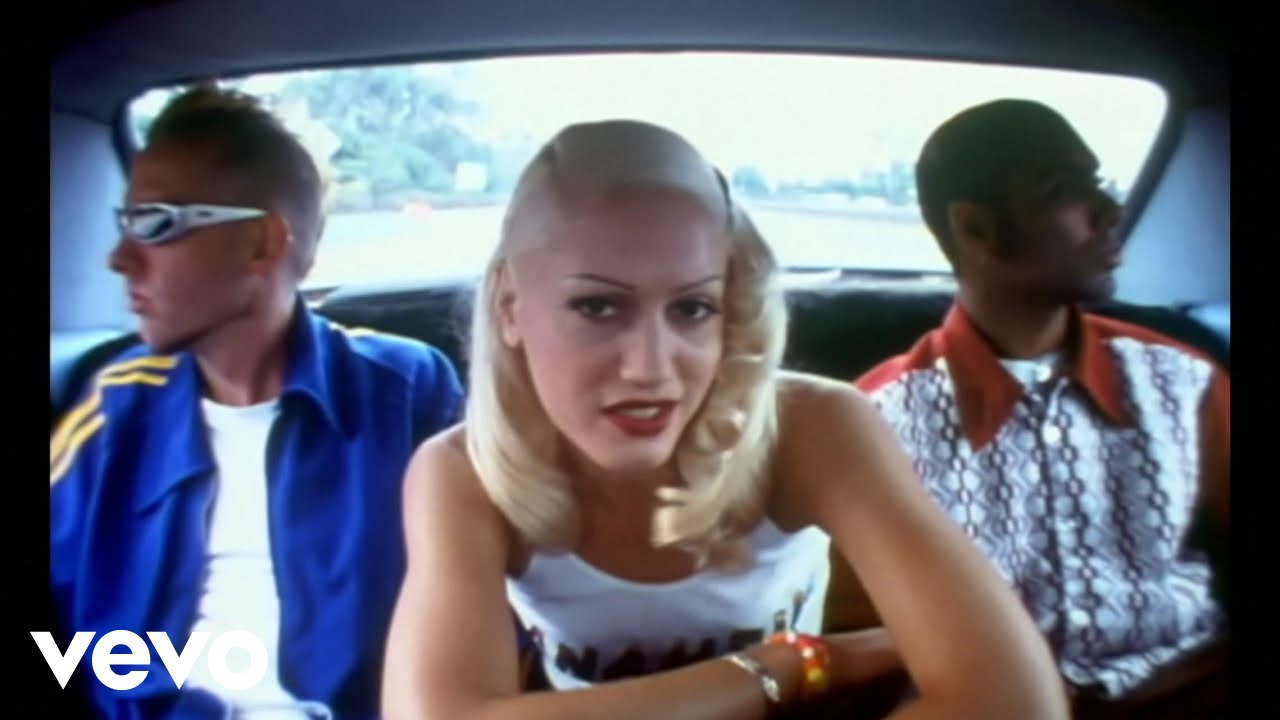
\includegraphics[keepaspectratio]{img/no-doubt.jpg}}

\begin{quote}
Girl's gotta eat.

---Alex Quicho, ``Everyone is a Girl Online''
\end{quote}

What are the available modalities of female identity circulating on
social media in 2024?

This is a question that I wanted to explore this week. It's a question
about gender, but a question more specifically about constructions of
\textbf{female} identity on contemporary social media platforms. As Alex
Quicho's reference to Andrea Long Chu's book \textbf{Females} (2018)
makes clear, even the idea of what ``female'' itself means has become
disarticulated from its biological (that is anatomical) and social
(gender) moorings.

So what are some dominant modalities of femaleness and/or femininity in
online social environments today? In part they are cultural stereotypes
we are already familiar with. Here's the beginning of a word cloud that
you can contribute your own entries to:

angel complex • bimbos • influencers • Karens • Barbie • beautiful
princess disorder (BPD) • SAWs • soccer moms • mom jeans • mukbang
(Korean food bloggers) • Japanese
\href{https://restofworld.org/2021/vtubers/}{VTubers} • I'm literally
just a girl • wanghong (Chinese influencers) • Xiaoyongshu girls •

The two articles that I assigned for us to discuss this week offer more
systematic and arguably contradictory answers to our opening question:
on the one hand, the cult of the Young-Girl (Tiqqun's concept,
referenced and updated by Alex Quicho); on the other, the Sexy Adult
Woman (SAW) modality that is challenged by what Emma Copley Eisenberg
calls Frump. Here's a good example (right margin) of the kind of value
that's attached to the word in mainstream culture, and from which
Eisenberg wants to rescue it.

\marginnote{\begin{footnotesize}

\href{https://nowthaticando.com/}{\pandocbounded{
\includegraphics[keepaspectratio]{img/frump-fighters.png}}}

\end{footnotesize}}

Incidentally, if you're looking for summer reading recommendations for
after the course is over, Emma Eisenberg has just published a novel,
\emph{Housemates}, that's supposed to be very good.

\marginnote{\begin{footnotesize}

\href{https://www.penguinrandomhouse.com/books/671798/housemates-by-emma-copley-eisenberg/}{\pandocbounded{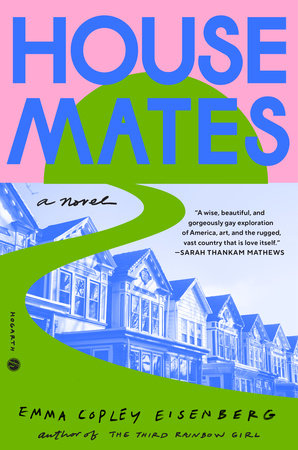
\includegraphics[keepaspectratio]{img/housemates.jpeg}}}

\end{footnotesize}}

I'm of course very curious to hear your own responses to these two
articles, for the moment will limit myself to just a couple of
observations that may help to get our discussion going. I've also
included a Resources section at the end of today's lecture, which has
links to multiple topics either referenced in the main readings or are
related to them. If you are interested in focusing on gender in social
media for your research project, these links may help you to narrow down
and focus on something specific within the very large field of gender
online.

\subsubsection{Beautiful Princess
Disorder}\label{beautiful-princess-disorder}

Perhaps the most conceptually intriguing point to come out of Alex
Quicho's article is that of the girl as a form of collective identity or
\textbf{networked subjectivity}. In particular, the frequent references
to \textbf{girl swarms} of course takes us back to Byung-Hul Han's
chapters from his book \emph{In the Swarm} that we were discussing a few
weeks back. I'm thinking in particular of passages like this one, which
references a few TikTok accounts:

\begin{quote}
Recently, some popular accounts
(@chloe21e8\marginpar{\begin{footnotesize}{?quarto-cite:chloe21e8}\vspace{2mm}\par\end{footnotesize}},
@lilclearpill\marginpar{\begin{footnotesize}{?quarto-cite:lilclearpill}\vspace{2mm}\par\end{footnotesize}},
and
@heartlocketxo\marginpar{\begin{footnotesize}{?quarto-cite:heartlocketxo}\vspace{2mm}\par\end{footnotesize}}
are personal favorites, though~it's more useful to read these as nodes
in a swarm rather than the products of any one mind) have struck a
collective nerve with their embodiment of an ever-shifting mass voice
that is ecstatic, girl-coded, and unknowable. ``I'm so mentally stable
it's insane.~I have BPD, beautiful princess disorder. I'm so
clear-pilled, I can see through the matrix. I'm not left-wing or
right-wing, I have angel wings that grow whenever I transcend into
space,''
goes~\href{https://www.tiktok.com/@basedredactedgang/video/7257143957312802053}{the
swarm thinking}~that has transcended format, individual creator, and
platform to
become~\href{https://www.tiktok.com/music/original-sound-7257143960665606918}{viral
TikTok
audios},~\href{https://www.instagram.com/reel/Cvx2c8primP/}{million-view
Reels},~\href{https://twitter.com/Grimezsz/status/1691229470844493824}{Grimes
citations}, and beautiful-princess Bible verses carved into my brainstem
like lovers' initials in a tree trunk.
\end{quote}

There are some key differences between Han's and Quicho's framing of the
swarm here. First, for Han, the swarm is an entirely negative
consequence of networked communication, producing the kind of
scapegoating and shaming culture discussed in the book \emph{The Shame
Machine}. By contrast, Quicho is pretty upbeat about the emancipatory
possibilties of the girl swarm and presents the idea of the girl as a
kind of ``hive mind'' in which individual identity is eclipsed by a
wider network subjectivity. If you have any immersion in platforms like
Instagram and TikTok you will have an idea of what she means.

Crucially, for Han social media is a world of \emph{dis}connected,
atomized \textbf{individuals}, in contrast to the anonymous effacement
of individuals in the modern \textbf{crowd}. For Quicho, social media is
the opposite. Or at least, to paraphrase Joe Jackson, It's Different for
Girls\ldots{}

\subsubsection{Post-Platform}\label{post-platform}

You may have noticed a few references to the term \textbf{post-platform}
in Alex Quicho's article, and may have been wondering about that.
\href{https://kylechayka.substack.com/p/the-post-platform-internet}{This
Substack article} by Kyle Chayka will help with that, but the main thing
to be aware of is that the term itself is now widely regarded as
discredited by the emerging new social mediascape. To get a better sense
of this, take a look at Sarah Marshall's recent prediction of how
``\href{https://www.niemanlab.org/2023/12/we-get-past-post-platform/}{We
get past `post-platform'},'' which provides an interesting snapshot of
the rapid transformations underway in today's social mediascape. Looking
through her list, it's hard to disagree that Chayka's melancholy
diagnosis of the demise of legacy SM platforms is premature, along with
the term ``post-platform'' itself. Something new is undoubtedly
emerging, as we'll be discussing in the remaining weeks of the course,
but even though the future looks more decentralized, social media
platforms are clearly not going the way of the dinosaurs anytime soon.

\subsubsection{Resources}\label{resources}

\href{https://www.instagram.com/frumpenberg/}{frumpenberg}~(ECE's
Instagram)

\href{https://emmacopleyeisenberg.substack.com/p/welcome-to-frump-feelings-b6e}{Frump
Feelings}~(ECE's Substack blog)

\textbf{Babygirls}

``\href{https://www.theguardian.com/lifeandstyle/2024/jan/24/so-babygirl-its-the-new-gen-z-term-of-endearment-but-what-does-it-mean}{So
babygirl! It's the new gen Z term of endearment -- but what does it
mean?}'' (\emph{The Guardian}, 24 January 2024).

Gita Jackson,
``\href{https://www.polygon.com/23711849/succession-babygirl-kendall-roy-jesse-breaking-bad}{Why
sad TV men are the internet's `babygirls'}'' (\emph{Polygon}, 8 May
2023).

Alaina Demopoulos,
``\href{https://www.theguardian.com/lifeandstyle/2022/oct/30/sadness-is-a-trend-why-tiktok-loves-crying-makeup}{`Sadness
is a trend': why TikTok loves `crying makeup'.}'' (\emph{The Guardian},
31 October 2022).

\begin{center}\rule{0.5\linewidth}{0.5pt}\end{center}

\textbf{\#MorningRoutine}

Rachel Signer,
``\href{https://www.theguardian.com/lifeandstyle/2023/feb/19/broadcasting-your-breakfast-why-tiktokers-obsess-over-morning-routines}{Broadcasting
your breakfast: why TikTokers obsess over morning routines}'' (\emph{The
Guardian}, 18 February 2023).

\begin{center}\rule{0.5\linewidth}{0.5pt}\end{center}

\textbf{Amalia Ulman}

\href{http://amaliaulman.eu/}{Website}

\href{https://www.instagram.com/amaliaulman/}{Instagram}

Alastair Sooke,
``\href{http://www.telegraph.co.uk/photography/what-to-see/is-this-the-first-instagram-masterpiece/}{Is
This The First Instagram Masterpiece?}'',~\emph{The Telegraph}, 18
January 2016

``\href{http://www.dazeddigital.com/artsandculture/article/23700/1/amalia-ulman-meme-come-true}{Amalia
Ulman: Meme Come True}'' (\emph{Dazed})

Emilie Friedlander,
``\href{http://www.thefader.com/2014/11/07/social-anxiety-why-amalia-ulmans-middlebrow-instagram-feed-is-no-different-from-yours}{Social
Anxiety: Why Amalia Ulman's Fake `Middlebrow' Instagram Is No Different
From Yours}'',~\emph{Fader}, 7 November 2014.

\begin{center}\rule{0.5\linewidth}{0.5pt}\end{center}




\end{document}
